% Шаблон для отчетов пол лабораторным работам в СПбГЭТУ "ЛЭТИ"
% Ефремов М.А. 2017г
%=== Тип документа - статья, кегль 14пт.
\documentclass[14pt]{article}
%=== Настройка кодировок, шрифта и языка
\usepackage[utf8]{inputenc}
\usepackage{extsizes}
\usepackage[main=russian, english]{babel}
\usepackage[T2A, T1]{fontenc}
%=== Разметка документа
\usepackage{geometry} 
\geometry{
	a4paper, 
	top = 2cm,
	bottom = 2cm,
	left = 3cm,
	right = 1cm
}
%=== Форматирование текста
\usepackage {setspace}			% Интерлиньяж
\onehalfspacing					% 1.5 строки
\usepackage {indentfirst} 		% Красная строка с первого предложения
\setlength						% Отступ красной строки - 1.25см
	{\parindent}
	{1.25cm}	
\usepackage {titlesec}			% Форматирование заголовков
% разделов
\titleformat
	{\section}
	[hang]
	{\normalsize\bfseries}
	{}{0pt}{}
\titlespacing
	{\section}
	{\parindent}
	{4ex}
	{0pt}
% подразделов (нумеруются)
\titleformat
	{\subsection}
	[hang]
	{\normalsize\bfseries\itshape}
	{\arabic{subsection}. }{0pt}{}
\titlespacing
	{\subsection}
	{\parindent}
	{4ex}
	{0pt}
%=== Минимизируем количество переносов
\usepackage {ragged2e}
\usepackage {microtype}
\tolerance = 500
\hyphenpenalty = 20000
\emergencystretch = 1cm
%=== Таблицы
\usepackage {tabularx}	% основной тип таблиц, выравнивание по ширине
\usepackage {longtable}	% для таблиц, не вмещающихся на одну страницу
\usepackage {multirow}	% для разбиения ячеек на несколько строк
\usepackage {multicol}	% на несколько колонок
%=== ^ до этого места - минимальная преамбула документа.
%=== Далее идут опциональные, но часто использущиеся пакеты,
%=== а так же написанные мной команды, чем-то упрощающие написание отчетов

%=== Работа с формулами
% Набор пакетов, сильно расширяющих возможности по набору формул
\usepackage{amsmath}
% добавляет специфические для русских  статей мат. символы вроде \leqslant
\usepackage{amssymb}
% добавляет окружения для теорем и лемм	
\usepackage{amsthm}				
\usepackage{mathtools}
% номера только для тех формул, на которые есть ссылки в тексте
\mathtoolsset{showonlyrefs=true}

%=== Работа с изображениями
\usepackage{graphicx}
\usepackage{caption}
\usepackage{subcaption}

%=== Работа с гиперссылками
\usepackage{hyperref}
\hypersetup{
	colorlinks=true,
	urlcolor=blue,
	filecolor=green,
	linkcolor=red
}

%=== Вставка кода
\usepackage{listings}
\usepackage{xcolor}
\lstset { %
	basicstyle = \footnotesize,% basic font setting
	captionpos = b,
	numbers    = left,
	frame      = single
}

% Компиляция под Windows 10 при помощи XeLaTeX для использования шрифта Times New Roman
\usepackage{fontspec}
\setmainfont{Times New Roman}

\begin{document}
	\pagenumbering{gobble}
\clearpage
\begin{center}	
	МИНОБРНАУКИ РОССИИ\\
	САНКТ-ПЕТЕРБУРГСКИЙ ГОСУДАРСТВЕННЫЙ\\
	ЭЛЕКТРОТЕХНИЧЕСКИЙ УНИВЕРСИТЕТ\\
	«ЛЭТИ» ИМ. В.И. УЛЬЯНОВА (ЛЕНИНА)\\
	Кафедра МО ЭВМ

	\vspace{54mm}

	ОТЧЕТ\\
	по лабораторной работе №1 \\
	по дисциплине «Алгоритмы компьютерного зрения» \\
	Тема: калибровка камеры \\

	\vspace{65mm}

	\def\arraystretch{1.5}
	\begin{tabularx}{\textwidth}{ >{\hsize=7cm}X >{\hsize=4.1cm}X  >{\centering\arraybackslash}X }
		Студент гр. 2304 & & Ефремов М.А. \\ \cline{2-2}
		Преподаватель & & Черниченко Д.А. \\ \cline{2-2}
	\end{tabularx}
	\def\arraystretch{1}

	\vfill
	Санкт-Петербург\\
	2017
\end{center}
\newpage
\pagenumbering{arabic}
\setcounter{page}{1}
	
	\section{Цель работы.}
		При помощи библиотеки OpenCV, используя предложенные изображения в качестве входных данных, получить карту глубины.
	
	\section{Основные теоретические положения.}
		На рисунке \ref{img:pipeline} показана реализация класса Stitcher библиотеки OpenCV, отвечающий за выполнение сшивающего конвейера. Используя этот класс можно управлять этапами выполнения конвейера.

\begin{figure}[h!]
	\includegraphics[width = \linewidth]{img/pipeline}
	\caption{схема работы сшивающего контейнера, реализованного в классе Stitcher.}
	\label{img:pipeline}
\end{figure}

Стоит отметить, что это общая последовательность работы класса Stitcher. Данная схема была взята из документации к версии OpenCV 2.4 со ссылкой на статью: Brown and D. Lowe. Automatic Panoramic Image Stitching using Invariant Features. International Journal of Computer Vision, 74(1), страницы 59-73, 2007 года.

В OpenCV 3.2, использовавшемся при выполнении работы, конвейер сохраняется и для построения панорамы выполняются примерно следующие шаги:

\begin{enumerate}
	\item Обнаружение ключевых точек (методы DoG, Harris, и т.д.) и описание локальных ориентиров (при помощи алгоритмов SIFT, SURF, и т.д.) по первым двум изображениям.
	\item Нахождение совпадений описаний ориентиров между двумя изображениями.
	\item \label{it:hom_matrix} Использование алгоритма RANSAC (RANdom SAmple Consensus — стабильный метод оценки параметров модели на основе случайных выборок) для оценки матрицы гомографии используя вектора описаний совпавших ориентиров.
	\item Применение деформирующих преобразований, используя матрицу гомографии, найденную на шаге \ref{it:hom_matrix}.
\end{enumerate}

Основная разница между реализацией Stitcher в OpenCV 2.4 и 3.2 в методах обнаружения ключевых точек и описаний локальных ориентиров (таких как SIFT и SURF).
	
	\section{Программа.}
		\input{tex/program}
		
	\section{Экспериментальные результаты.}
		Для создания панорамы использовались фотографии, приведенные на рисунке \ref{img:input_imgs}, а результат работы написанной программы приведен на рисунке \ref{img:result}.

\begin{figure}[h!]
	\center {
		\includegraphics[width=\linewidth / 2, angle = -90]{img/left} \vspace{5mm}
		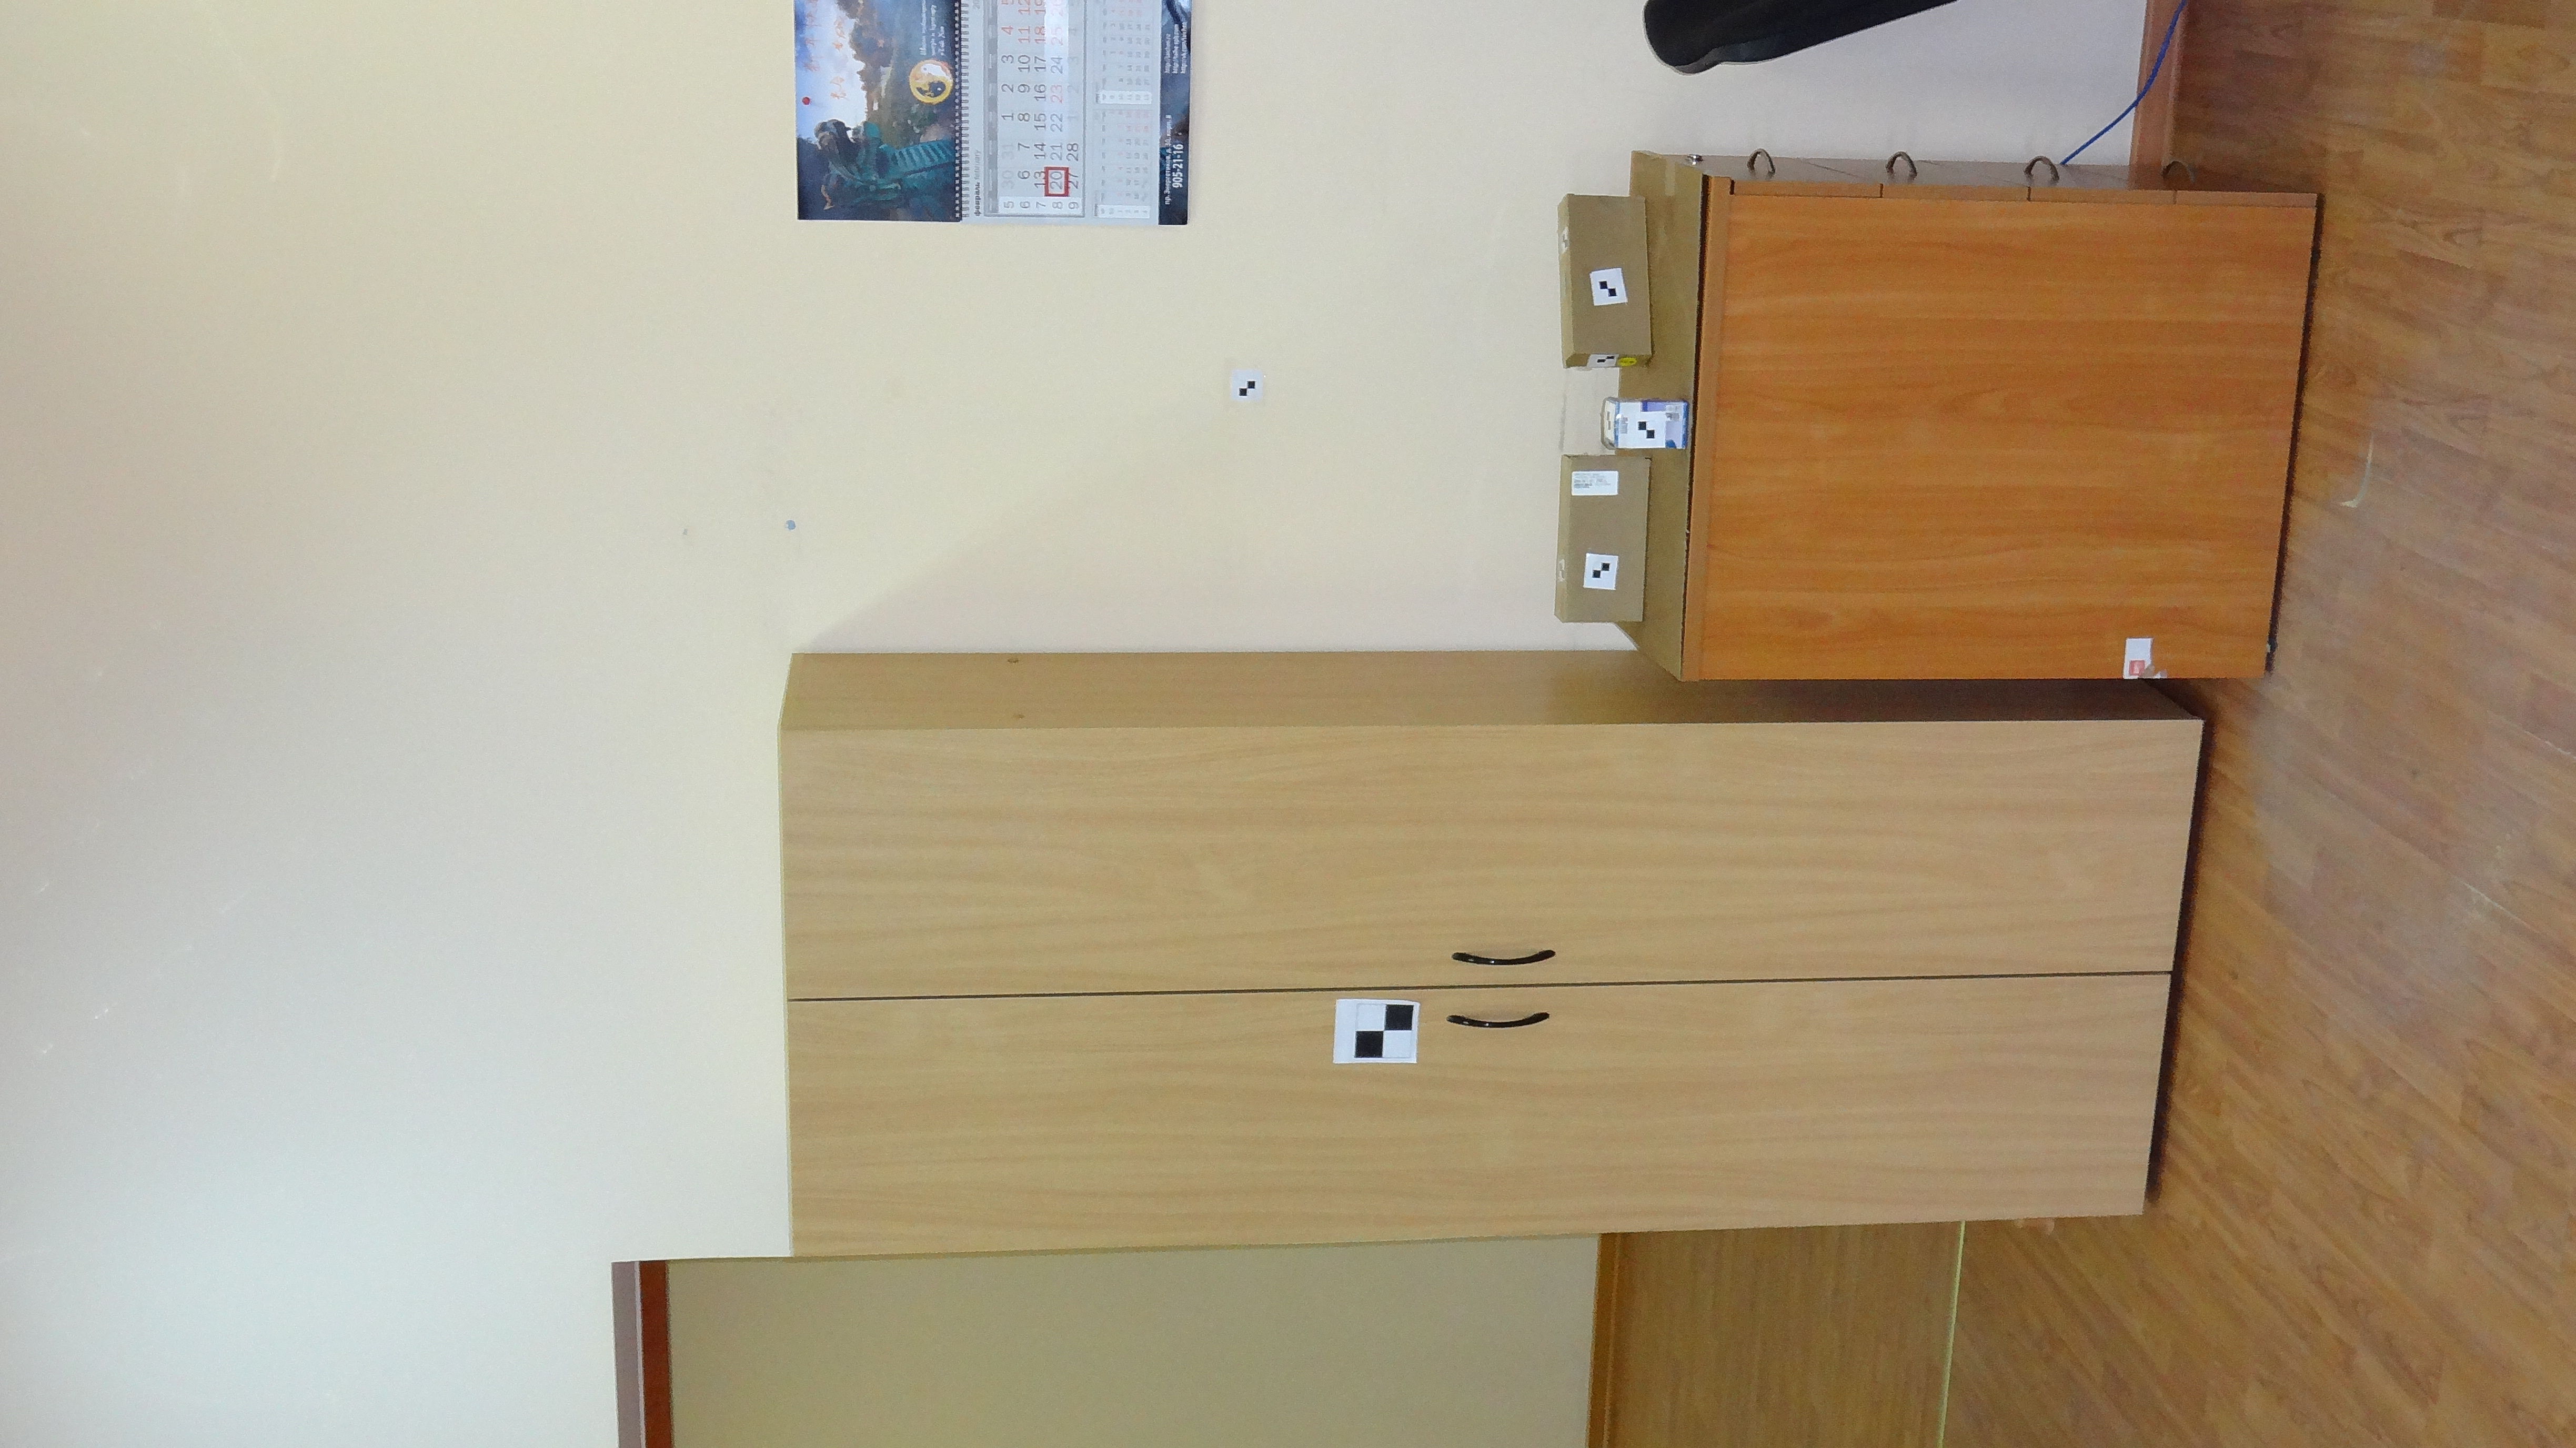
\includegraphics[width=\linewidth / 2, angle = -90]{img/right}
	}
	\caption{Фотографии для создания панорамы}
	\label{img:input_imgs}
\end{figure}

\begin{figure}[h!]
	\center {
		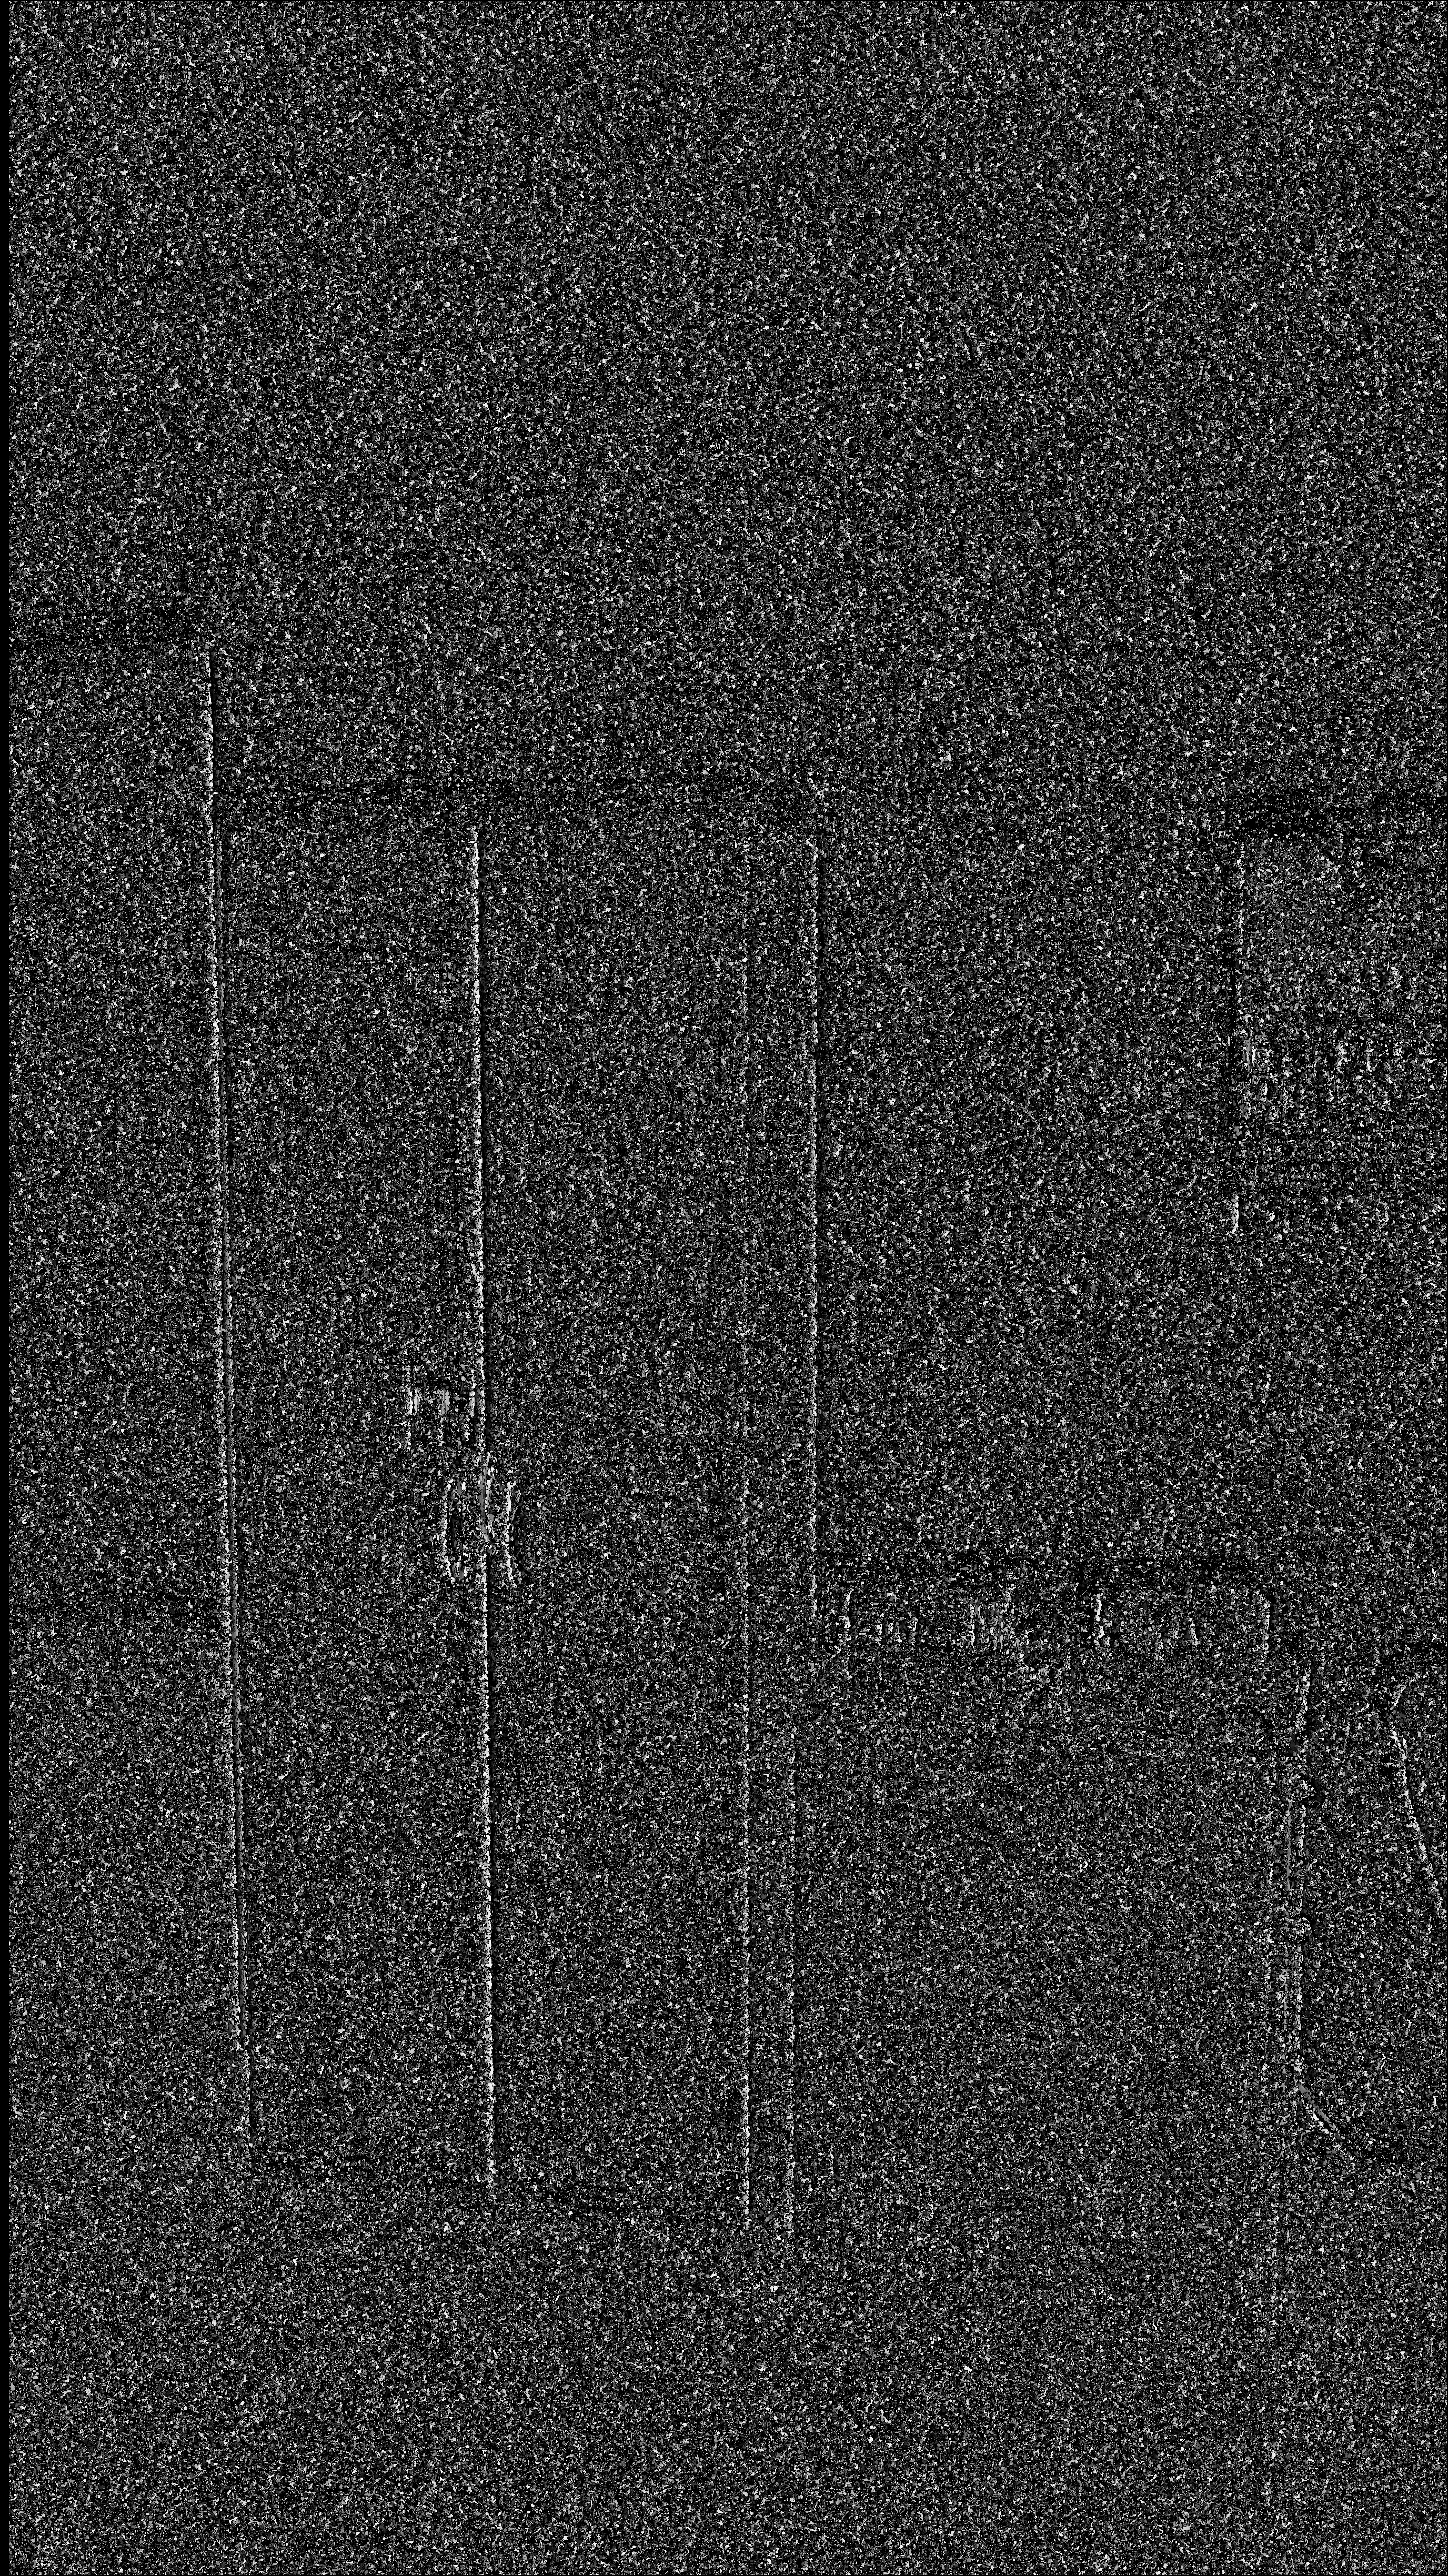
\includegraphics[width=\linewidth]{img/result}
	}
	\caption{Полученное изображение панорамы}
	\label{img:result}
\end{figure}

	\section{Выводы.}
		В результате выполнения программы была получена карта глубины, но, скорее-всего из-за большого расстояния до объектов, ее точность оставляет желать лучшего. т.к. явно более далекие объекты не всегда отличимы от близких. Ближайшие объекты шкаф и тумбочка и они находятся достаточно далеко от камеры.

\end{document}